\begin{figure}
  \centering
  \begin{subfigure}[b]{0.45\textwidth}
      \centering
      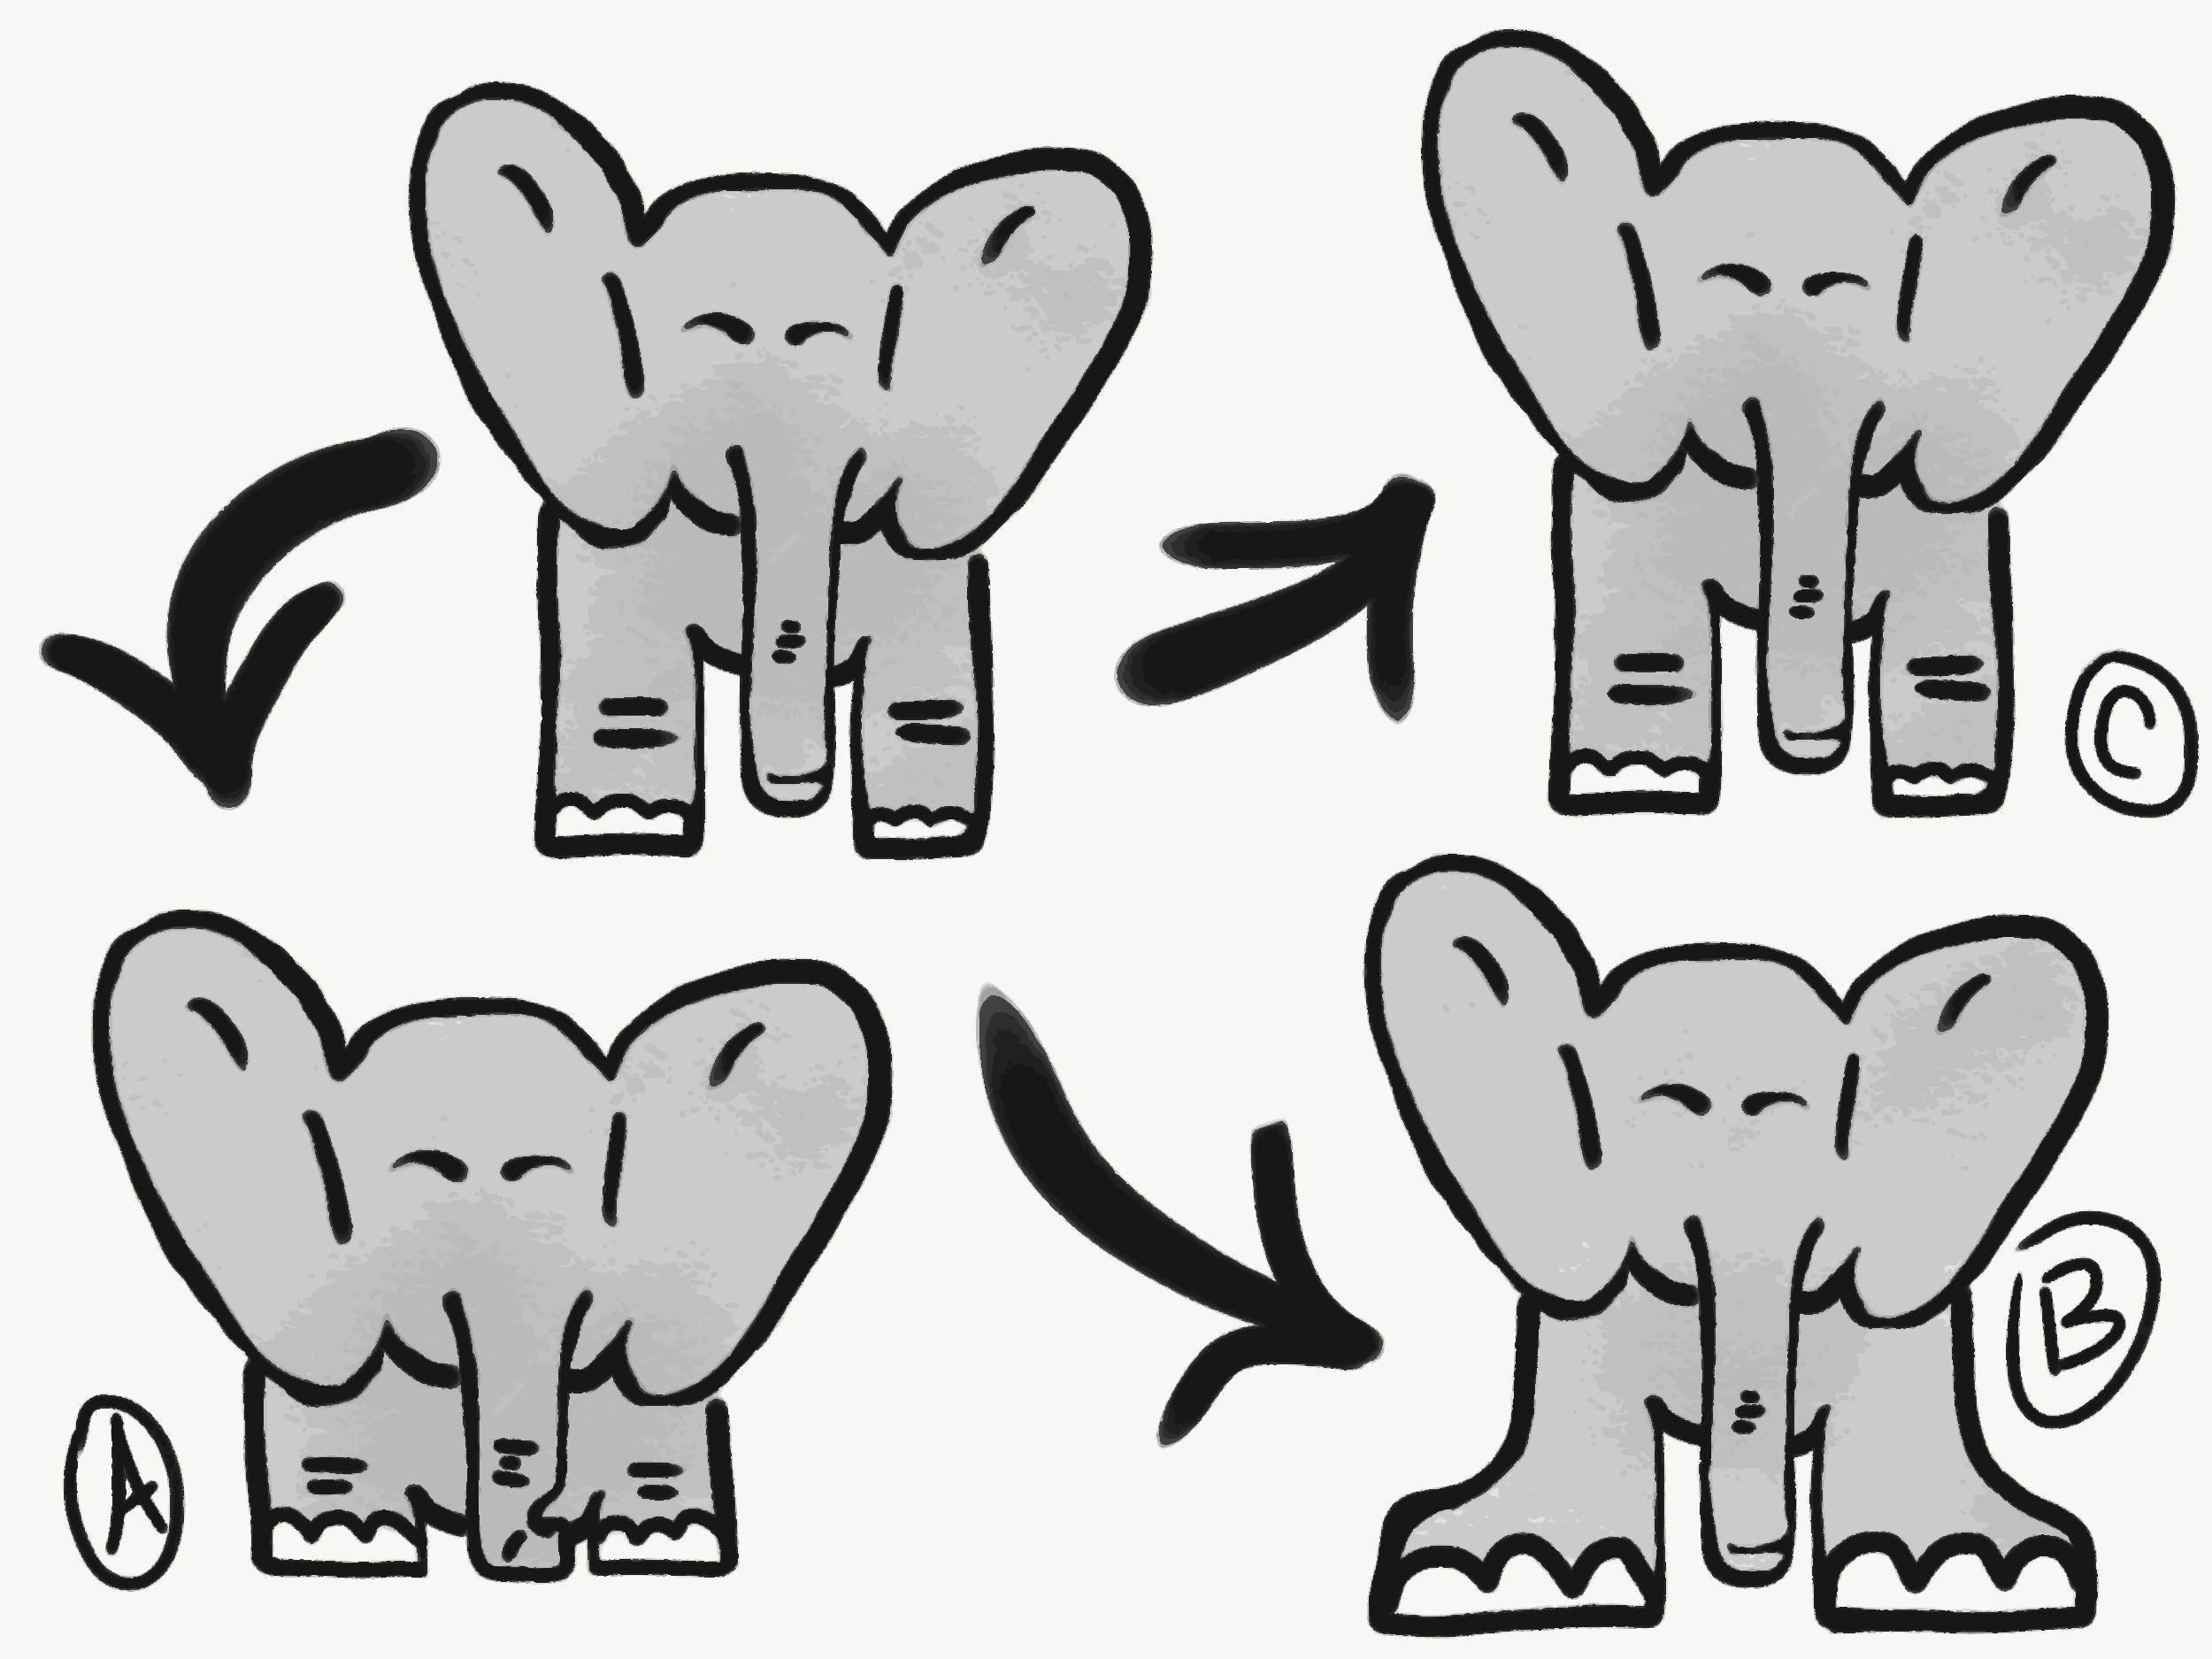
\includegraphics[width=\textwidth]{img/canalization_cartoon}
      \caption{canalization}
      \label{subfig:canalization}
    \end{subfigure}%
    \hfill
    \begin{subfigure}[b]{0.45\textwidth}
      \centering
      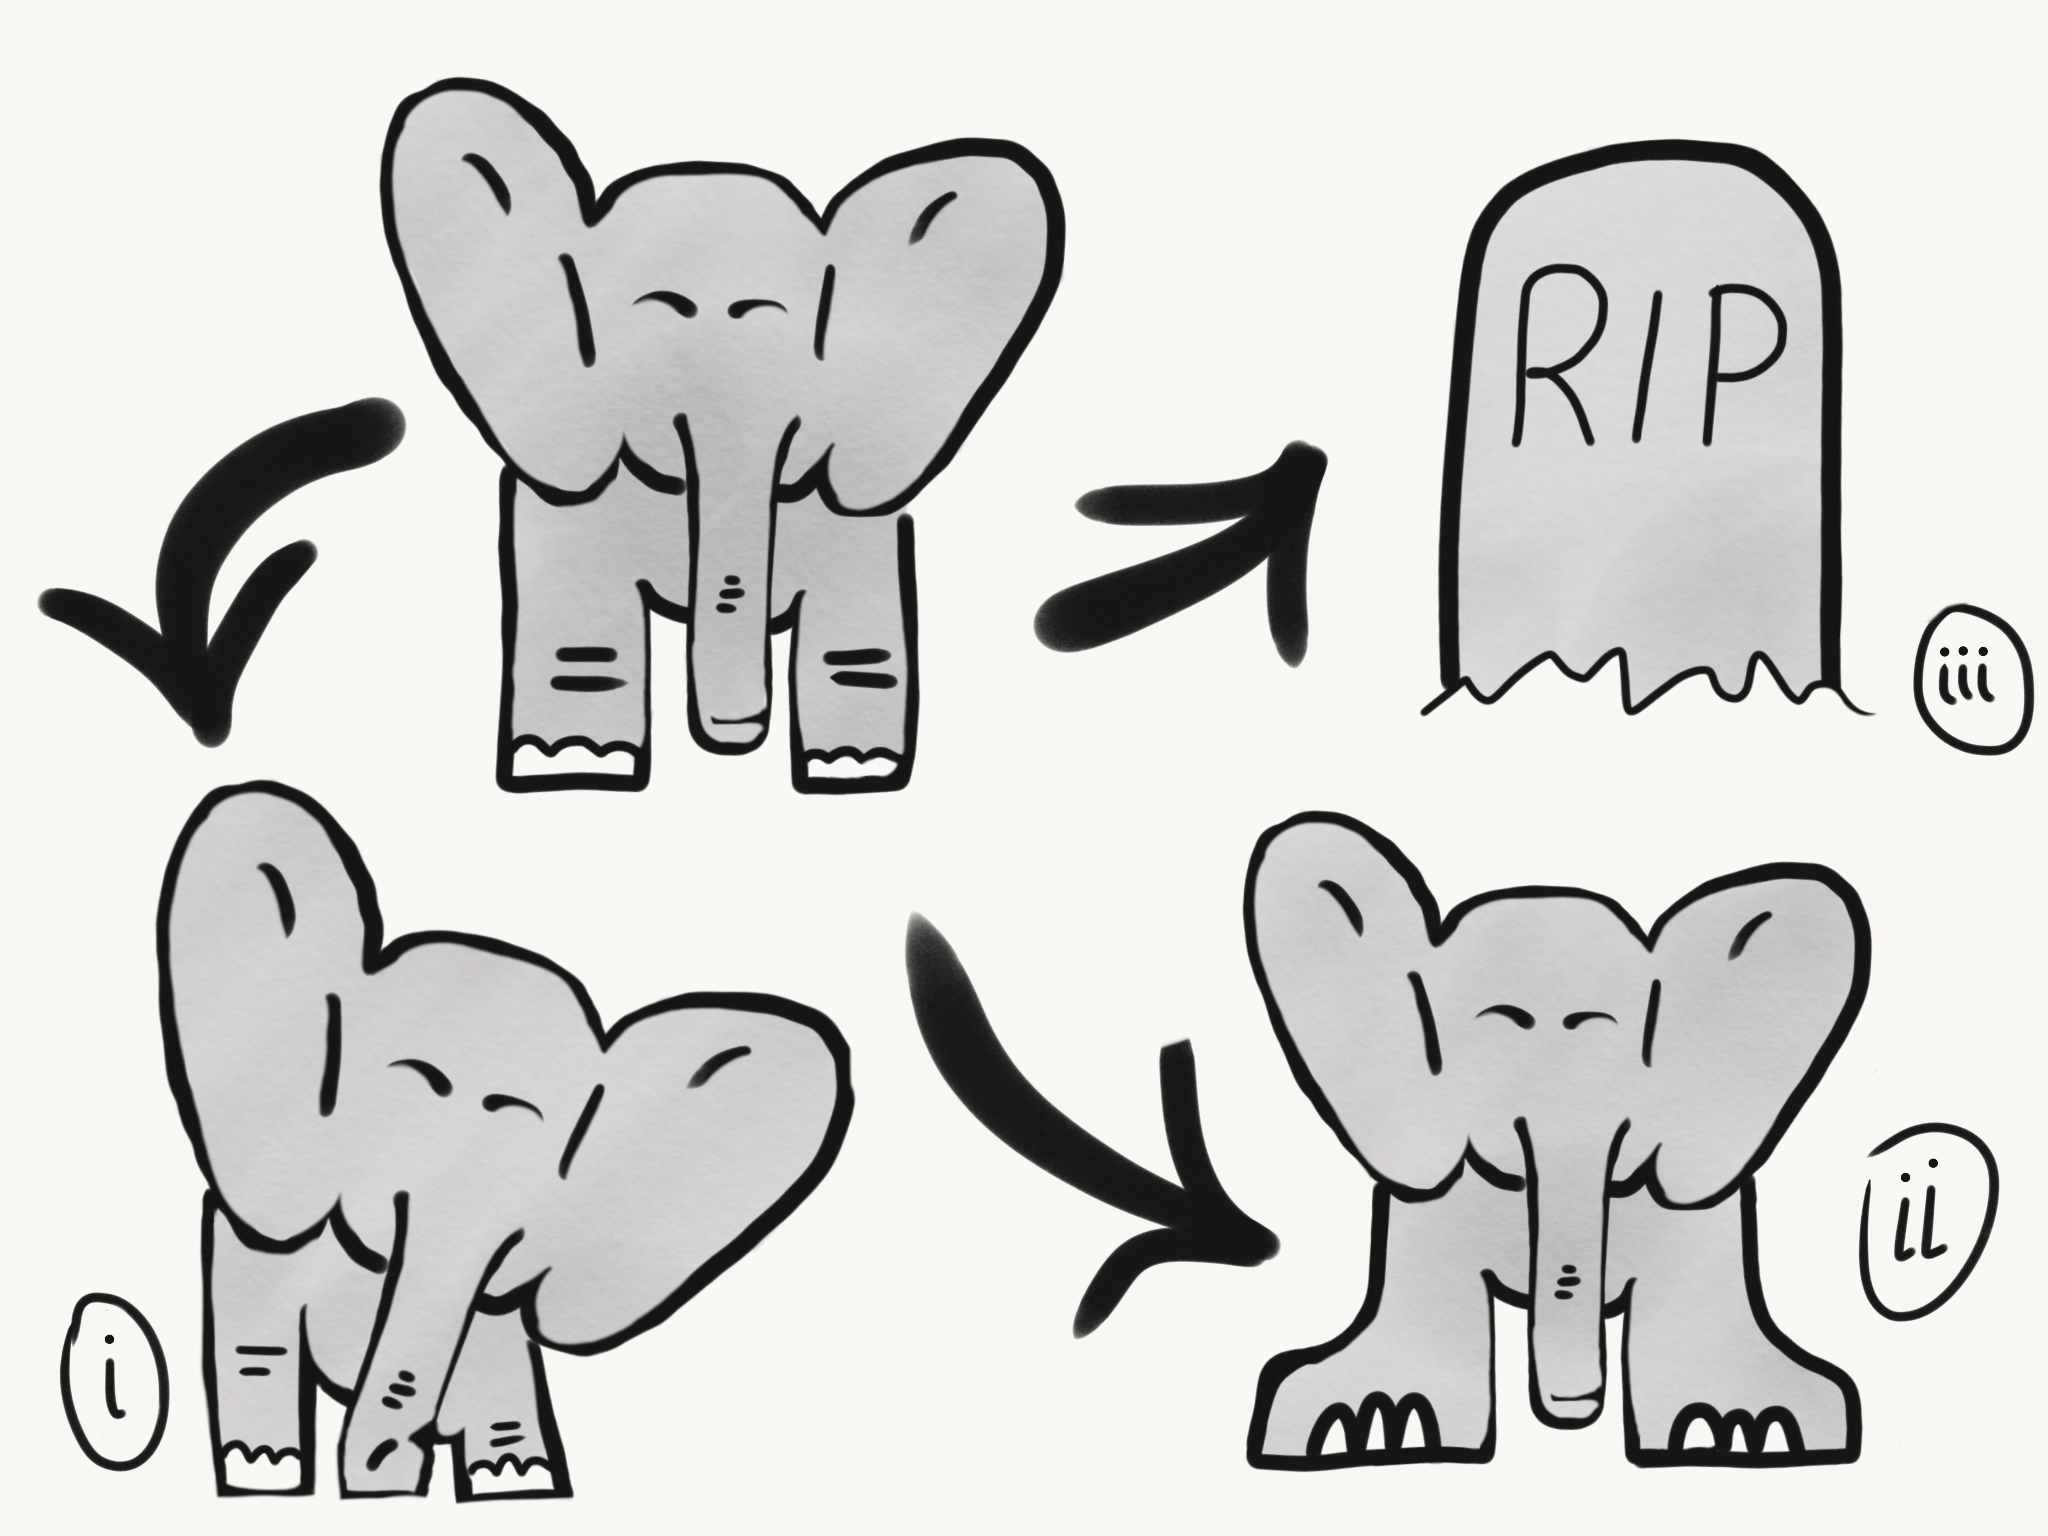
\includegraphics[width=\textwidth]{img/no_canalization_cartoon}
      \caption{non-canalization}
      \label{subfig:no_canalization}
    \end{subfigure}
 	\captionsetup{singlelinecheck=off,justification=raggedright}
  	\caption[A comparison of canalization and noncanalization]{a/i illustrates symmetry, b/ii illustrates grow-to-fit (exploratory growth \cite{Downing2015IntelligenceSystems}, c/iii illustrates robustness}
    \label{fig:canalization_vs_noncanalization}
\end{figure}